% !TeX program = xelatex
\documentclass[a4paper,11pt,lang=en,math=cm,bibend=bibtex]{elegantpaper}
\usepackage{array,tabularx}
\hypersetup{hidelinks,pdftitle={Human TFEB Cloning and Nutrient-Dependent Localization},pdfauthor={Siyuan Jiang and Ziyan Song}}
\linespread{1.15}
\setlength{\emergencystretch}{2em}
\addbibresource{references.bib}
\title{Cloning of Human TFEB and Analysis of Its Nutrient-Dependent Subcellular Localization in HeLa Cells}
\author{Siyuan Jiang \and Ziyan Song}
\institute{Molecular Biology Laboratory Course}
\version{Working draft}
\date{October 23, 2026}
\begin{document}
\maketitle
% Necessary A/B interface updated from P5-accepted construct values.
\begin{abstract}
Transcription factor EB (TFEB) is a nutrient-responsive regulator of autophagy and lysosomal biogenesis. This proposal connects a defined human TFEB cloning design to a HeLa-cell localization assay. The selected reporter is TFEB--EGFP, with EGFP at the C terminus of TFEB. Reconstruction from versioned source sequences yields a \ConstructBp{} bp design encoding \FusionAa{} residues, with an unmodified theoretical mass of \FusionMassKDa{} kDa. The proposed workflow uses high-fidelity PCR, HindIII/BamHI cloning into pEGFP-N1, bacterial screening, and complete fusion-region Sanger verification before cell use. The hypothesis is that starvation or Torin1 treatment increases reporter nuclear accumulation relative to the corresponding nutrient or solvent control. Fluorescence microscopy and anti-GFP immunoblotting will assess localization and expression. Sequence calculations are reported as in-silico checks; all experimental outcomes are predictions. The independent cell-assay details remain a part-A working draft.
\keywords{TFEB; autophagy; lysosome; mTORC1; EGFP fusion protein; subcellular localization}
\end{abstract}

% Owner A: Ziyan Song.
\section{Rationale and Research Basis}
TFEB is a member of the MiT/TFE transcription-factor family and a major transcriptional regulator of the autophagy--lysosome pathway. Under nutrient-rich conditions, mTORC1-dependent phosphorylation favors cytoplasmic retention of TFEB. During nutrient starvation or mTOR inhibition, TFEB accumulates in the nucleus and activates genes involved in lysosomal biogenesis and cellular clearance \cite{Settembre2012,RoczniakFerguson2012}. Nutrient-dependent control of nuclear export also contributes to TFEB distribution \cite{Napolitano2018}.

This project connects molecular cloning with a visible cell-biological phenotype. Its primary readout is the nuclear-to-cytoplasmic distribution of a fluorescent TFEB fusion. The study will test whether the sequence-verified reporter exhibits the expected nutrient-dependent redistribution in HeLa cells.

\subsection{Research Objectives and Hypothesis}
The first objective is to construct and sequence-verify an EGFP-tagged TFEB mammalian expression plasmid. The second is to compare its subcellular localization under normal culture, starvation, and mTOR-inhibitor conditions. The hypothesis is that starvation and mTOR inhibition increase the nuclear-to-cytoplasmic fluorescence ratio relative to the vehicle-treated control.

% Shared section structure. Edit the assigned method files independently.
\section{Experimental Design}
\subsection{Overall Workflow}
The study proceeds from reference-sequence retrieval and primer design to PCR amplification, plasmid construction, clone verification, transient transfection, and localization analysis. Sequence verification is the gate between molecular cloning and cell-based experiments.
% Owner B: Siyuan Jiang. Sequence-level design is not yet finalized.
\subsection{Construct Strategy and Materials}
The starting outline proposes an N-terminal EGFP--TFEB fusion expressed from a CMV promoter, using pEGFP-C1 as a candidate backbone. The final design will specify a single backbone and a versioned TFEB coding sequence, then verify the promoter, fusion junction, multiple cloning site, bacterial replication origin, and bacterial and mammalian selection markers. The original outline's fusion orientation remains provisional until the sequence and literature checks are complete.

For an EGFP--TFEB construct with TFEB at the C terminus, the TFEB termination codon should be retained unless an additional downstream fusion is explicitly intended. For the alternative TFEB--EGFP orientation, the native TFEB termination codon must be omitted to permit translation into EGFP. Removing a stop codon does not by itself establish the correct reading frame; both junctions require sequence-level verification.

The planned molecular materials are a defined human TFEB template, the selected EGFP expression vector, high-fidelity DNA polymerase, two compatible restriction enzymes, DNA ligase, competent \textit{Escherichia coli} DH5$\alpha$, and media containing the antibiotic specified by the verified backbone. A circular plasmid map will show the final sequence features and cloning junctions.

\subsection{Sequence Retrieval and Primer Design}
A human TFEB reference transcript and coding sequence will be retrieved from NCBI with accession and version recorded. Each cloning primer will be reported in the 5$'$ to 3$'$ direction and annotated by protective bases, restriction site, any frame-adjustment or linker bases, and template-annealing sequence. The selected enzyme pair must cut the intended backbone at the required positions without cutting the TFEB insert internally. Primer length, melting temperature, and compatibility with the amplification conditions will be documented after the sequence is fixed.

\subsection{PCR Amplification and Restriction Cloning}
The TFEB insert will be amplified with a high-fidelity polymerase. A no-template control and an appropriate amplification control will accompany the reaction. The intended amplicon will be purified, and both insert and vector will be digested and purified before ligation. An initial insert-to-vector molar ratio of approximately 3:1 is proposed. The ligation will be transformed into competent DH5$\alpha$ cells, followed by selection using the backbone's confirmed antibiotic marker. The reaction composition, thermal program, digestion conditions, and transformation details remain to be specified for the selected reagents.

\subsection{Clone Screening and Sequence Verification}
Candidate colonies will be screened by colony PCR and diagnostic restriction digestion. Plasmid DNA from positive clones will be purified for Sanger sequencing with vector-flanking and, where necessary, internal primers. A construct will be accepted only when the complete TFEB insert, both junctions, fusion reading frame, and terminal stop codon match the intended sequence without unintended substitutions, insertions, or deletions. An expected-size band alone will not establish sequence identity.

% Derived sequences are saved separately from the accepted WT design.
\subsection{Sequence-Defined Control and Mutant Constructs}\label{sec:control-constructs}
Five plasmid conditions are defined: parental pEGFP-N1 expressing EGFP only, the accepted WT TFEB--EGFP reporter, and three derived reporters carrying S211A, S142A or S142A/S211A (Figures~\ref{fig:control-plasmids} and \ref{fig:mutant-plasmids}). Amino-acid positions refer to human NP\_009093.1. The fusion constructs share the same 6,134-bp plasmid architecture, the GDPPVAT junction and C-terminal EGFP, and encode 722 residues. The two single mutants and their combination allow site-specific and combined comparisons; they are not three interchangeable ``constitutively nuclear'' positive controls~\cite{Vega2017,Napolitano2018}.

\begin{table}[htbp]
\centering\small
\caption{Exact designed codon changes; plasmid coordinates are 1-based inclusive.}
\begin{tabularx}{\textwidth}{l l l Y}
\toprule Variant & Codon change & Plasmid nucleotides & Comparison enabled \\
\midrule
S142A & AGC $\rightarrow$ GCC & 1054--1056 & Recovery with or without the S142 phospho-acceptor \\
S211A & TCC $\rightarrow$ GCC & 1261--1263 & S211-dependent distribution and 14-3-3 association \\
S142A/S211A & Both changes & Both intervals & Combined perturbation versus each single mutant \\
\bottomrule
\end{tabularx}
\end{table}

Generate each mutant using a sequence-defined synthetic donor with the same cloning flanks as the accepted WT amplicon, followed by the established HindIII/BamHI workflow. The supplied donor FASTAs specify the intended DNA; they are not purchased or experimentally validated material. Existing cloning primers may amplify the matched donors, but new mutagenesis primers are not invented. Include no-template PCR, digested-vector-only ligation and the established positive transformation control for each batch. Sequence the full fusion region and both junctions in both directions, explicitly including both target codons. Use two independently recovered, sequence-correct bacterial clones per genotype for key-contrast confirmation to detect clone/preparation-specific effects; randomize clone identity across experimental days. Bacterial clones are not additional biological cell-culture replicates.

The derived sequences retain the WT reading frame and unique HindIII/BamHI cleavage geometry. Ordinary diagnostic band sizes therefore do not identify these point mutants; the existing gel predictions apply to their gross insert/backbone sizes only. Sequence acceptance, intact expression and cell phenotype are three distinct checks. Alanine removes the serine phospho-acceptor but can also alter local interactions; none of these substitutions alone proves the responsible kinase or a direct phosphorylation reaction. A phosphomimetic S-to-D/E construct is not included as a guaranteed phosphorylated-state control.

\begin{figure}[htbp]
\centering
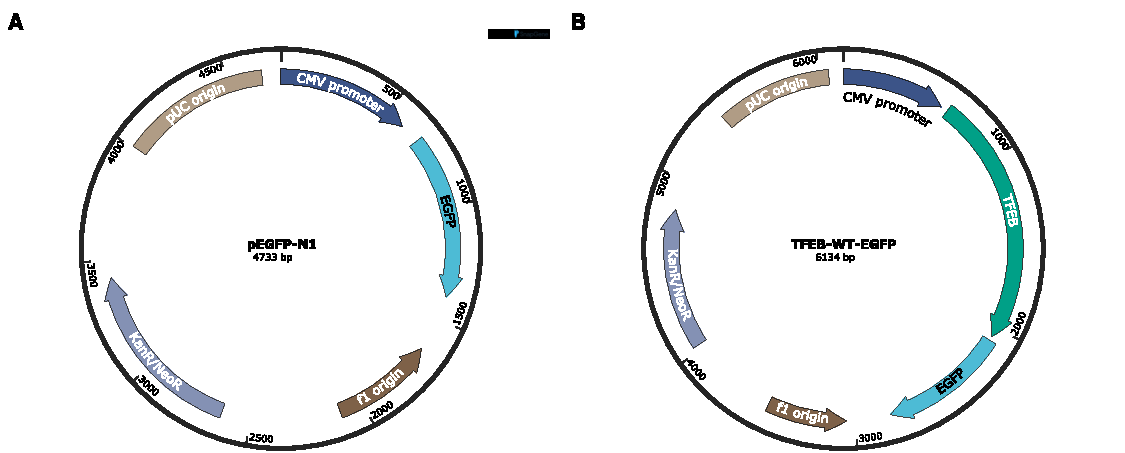
\includegraphics[width=\textwidth]{images/B/control-plasmids.pdf}
\caption{SnapGene Viewer maps of (A) the 4,733-bp EGFP-only control and (B) the 6,134-bp WT TFEB--EGFP reporter. Selected features retain their sequence coordinates and use a consistent NPG palette. The linker and minor regulatory annotations are omitted at this scale; complete GenBank records accompany the design. Native SVG geometry and vendor credit are preserved; the size unit is typeset in English. These are designed constructs, not verified experimental clones.}
\label{fig:control-plasmids}
\end{figure}

\begin{figure}[htbp]
\centering
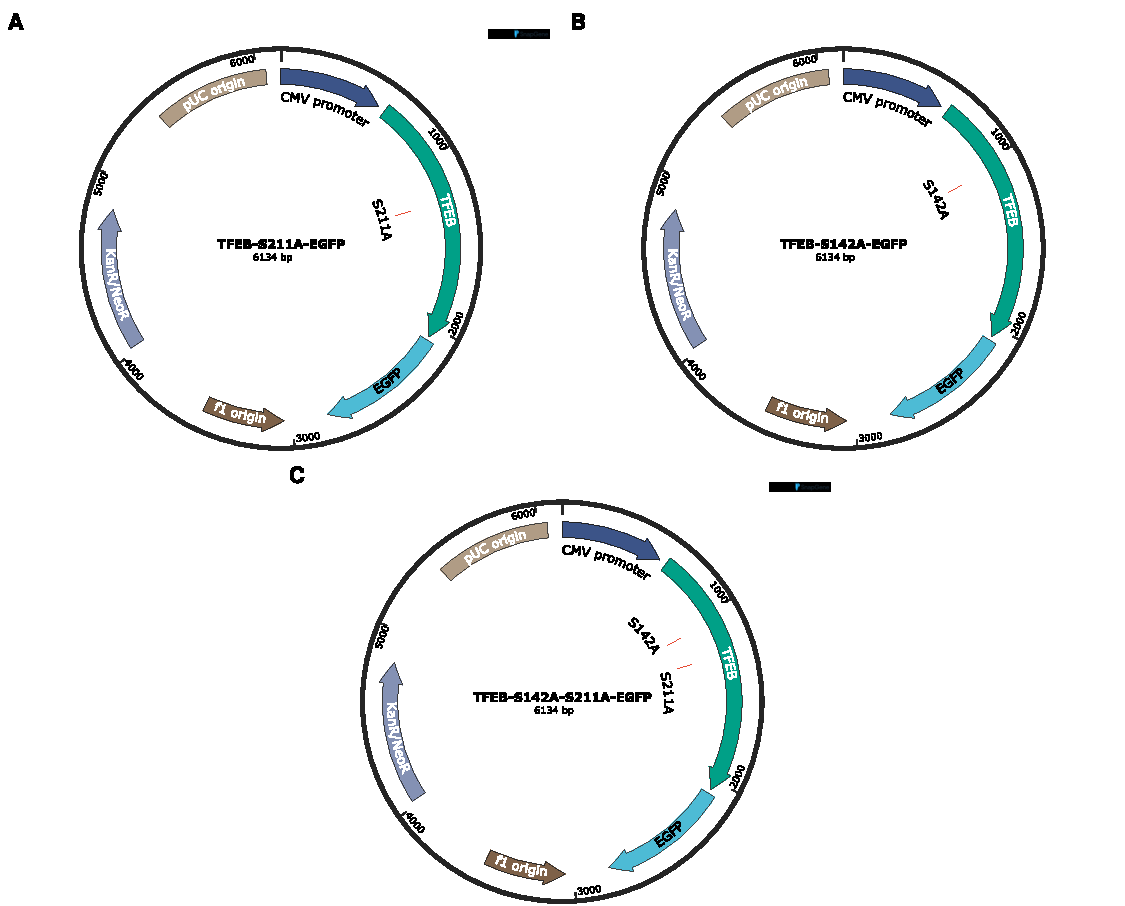
\includegraphics[width=0.98\textwidth,height=0.74\textheight,keepaspectratio]{images/B/mutant-plasmids.pdf}
\caption{SnapGene Viewer maps of (A) S211A, (B) S142A and (C) S142A/S211A. Red marks identify the substituted codons; residue numbering refers to NP\_009093.1. Every plasmid remains 6,134 bp and encodes 722 residues. EGFP, backbone and linker sequences remain identical to WT. These substitutions define experimental comparisons and do not establish a constitutively nuclear phenotype.}
\label{fig:mutant-plasmids}
\end{figure}
\FloatBarrier

% Owner A: Ziyan Song. Exact treatment and sampling parameters remain open.
\subsection{Cell Culture, Transfection, and Treatment}
After experimental sequence acceptance, \ConstructName{} (TFEB--EGFP) will be transiently transfected into HeLa cells. Starvation will be compared with time-matched nutrient-replete culture. Torin1-treated cells will be compared with nutrient-replete cells receiving the same final solvent concentration. The corresponding empty pEGFP-N1 (U55762.1; \EmptyVectorBp{} bp) will serve as the EGFP-only vector control; mock-transfected cells will define background. These controls will be included under the corresponding treatments. The final cell-assay protocol will identify the culture medium, transfection reagent, cell density, DNA amount, and treatment concentration and duration. These independent part-A parameters remain to be finalized; no cell experiment is claimed here.

\subsection{Imaging and Localization Analysis}
After treatment, cells will be fixed and counterstained with DAPI. Fluorescence images will be collected using consistent acquisition settings. Nuclear and cytoplasmic regions will be defined for each eligible transfected cell, and background-corrected mean fluorescence will be used to calculate the nuclear-to-cytoplasmic ratio:
\begin{equation}
R_{\mathrm{N/C}} = \frac{I_{\mathrm{nucleus}}-I_{\mathrm{background}}}{I_{\mathrm{cytoplasm}}-I_{\mathrm{background}}}.
\end{equation}
At least three independent experiments are planned. The number of cells per replicate, eligibility criteria, and handling of background-level cytoplasmic signals will be specified before analysis. Cells within one experiment will not be treated as independent biological replicates. The final statistical comparison will account for the experimental unit and the planned control-versus-treatment comparisons.

\subsection{Expression Validation}
An anti-GFP Western blot will assess expression of the \FusionAa{}-residue fusion and additional immunoreactive species. Its calculated unmodified average mass is \FusionMassKDa{} kDa, including the \LinkerPeptide{} linker. This value guides interpretation and is not an exact SDS-PAGE migration criterion: TFEB phosphorylation-dependent mobility shifts have been reported \cite{RoczniakFerguson2012}. The EGFP-only vector expresses the distinct \EGFPAa{}-residue tag product. A lower band in the fusion sample would prompt checks for cleavage or other products rather than an identity assignment from size alone. The final part-A protocol must specify lysis, loading amount/control, antibodies and detection conditions. Whole-cell immunoblotting assesses expression; the imaging assay establishes localization.

\subsection{Execution Plan and Deliverables}
The core program is organized into twelve modules with explicit outputs (Table~\ref{tab:workplan}). The timeline is a proposed eight-week allocation after reagent availability, not a record of work performed. Five additional research modules are specified separately in the next section. Modules advance only after their stated acceptance checks. Figure~\ref{fig:evidence-design} connects the different levels of evidence; arrows indicate the planned order of investigation, not demonstrated causation.

\begin{figure}[htbp]
\centering
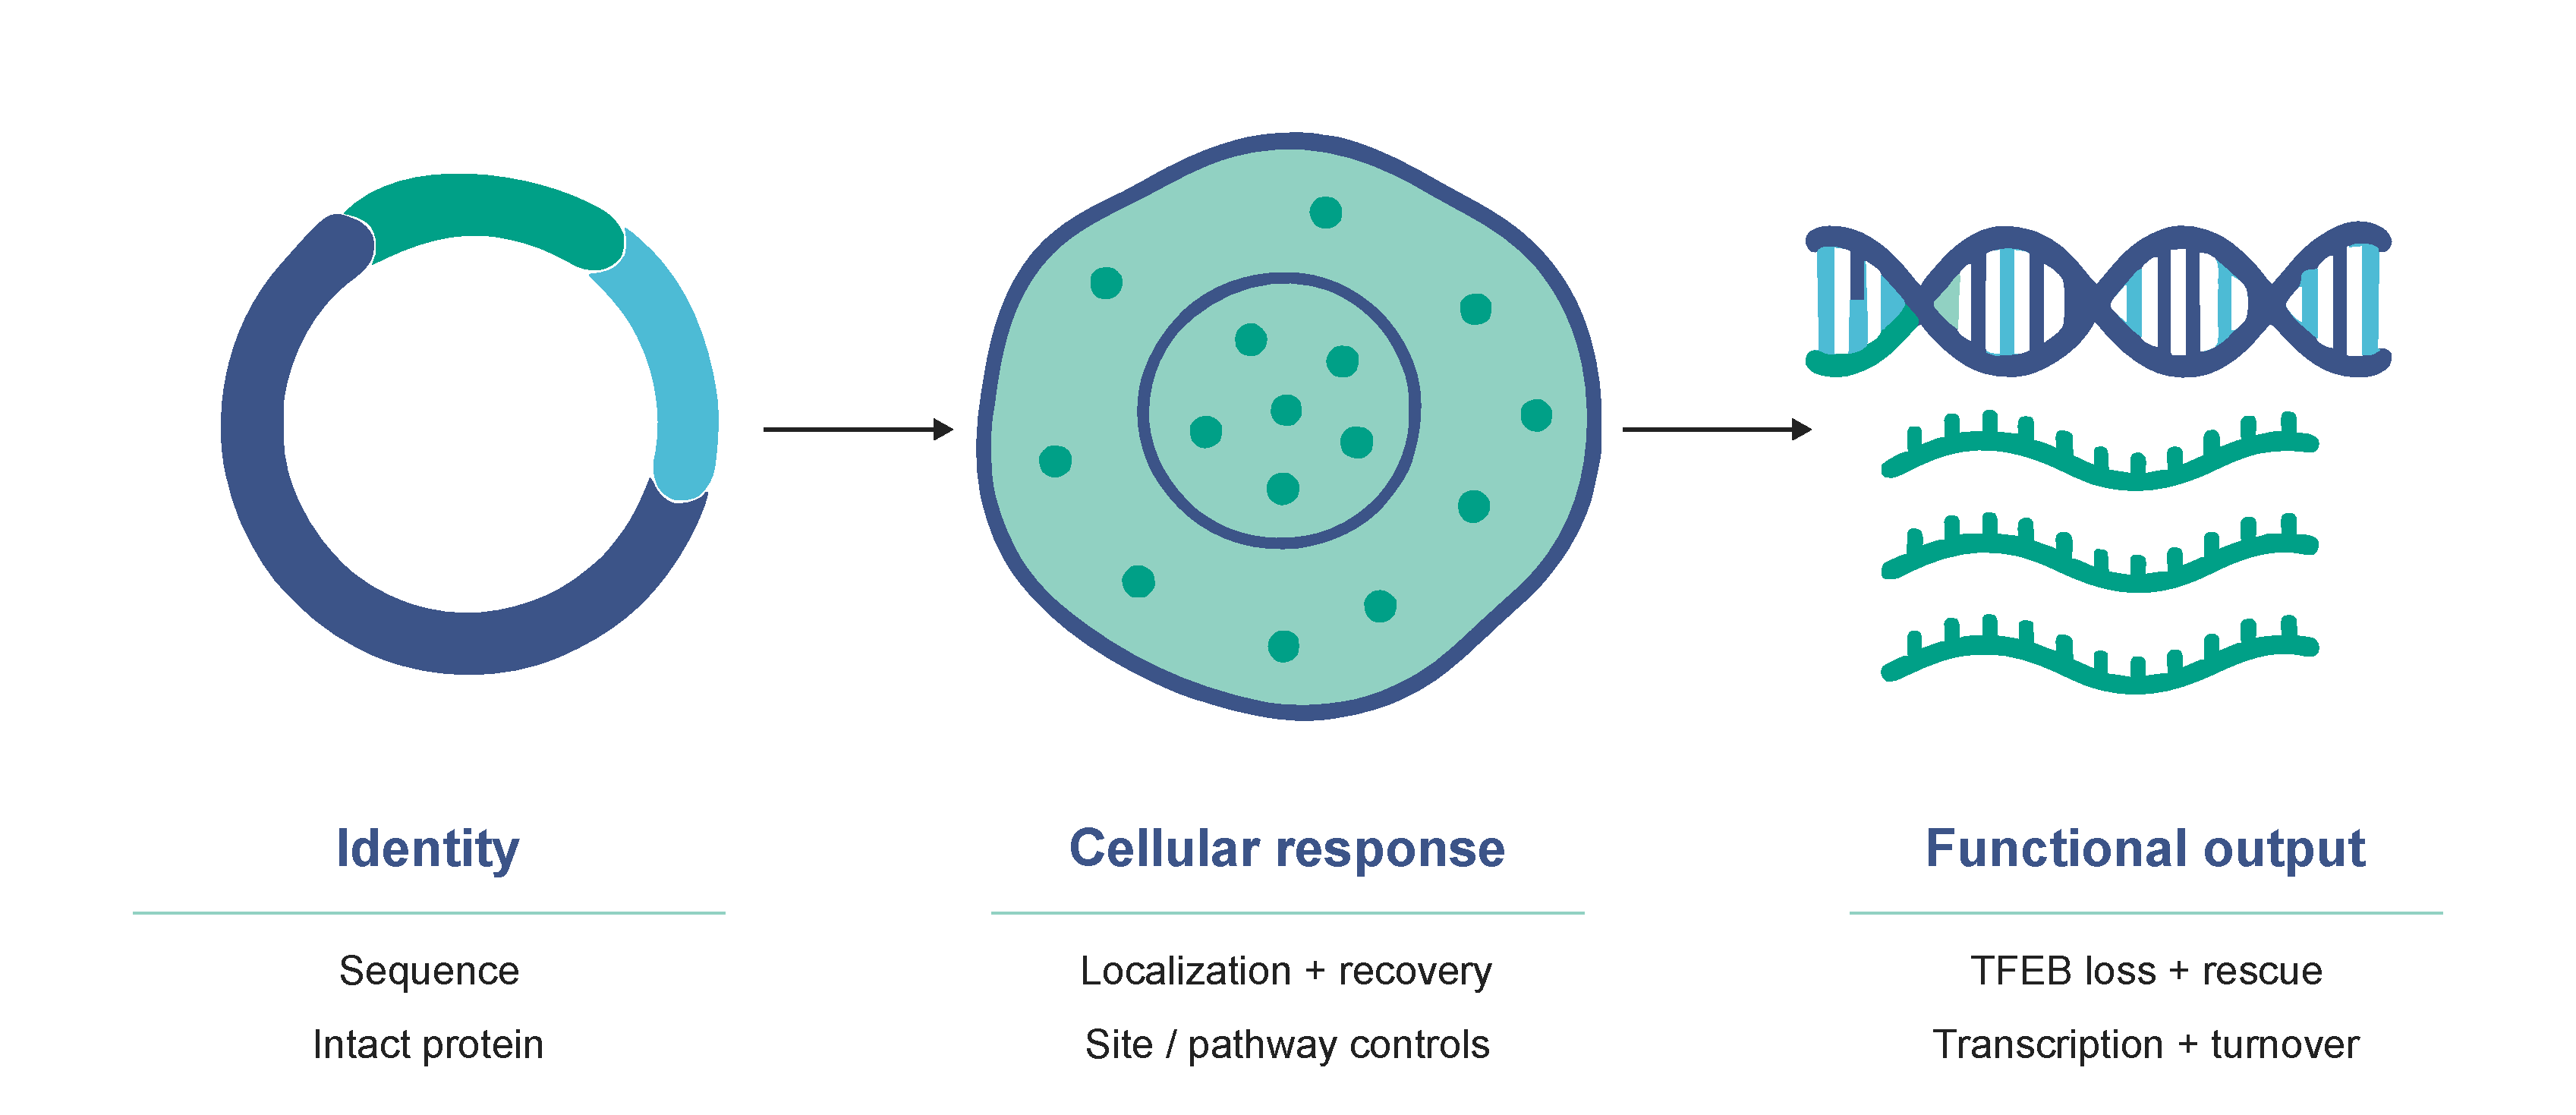
\includegraphics[width=\textwidth]{images/B/evidence-design-imagegen-v3.pdf}
\caption{Evidence structure for the expanded study. Construct identity precedes biological assays; reporter and endogenous localization are checked before site/pathway interpretation. TFEB loss/rescue tests target-gene RNA responses and turnover. The transcription branch requires qualified nascent-RNA evidence for a rate interpretation; turnover requires paired bafilomycin A1 controls. Icons are conceptual drawings, not experimental images. Each stage needs the negative, positive and specificity controls in the methods. Agreement strengthens interpretation; disagreement narrows the conclusion.}
\label{fig:evidence-design}
\end{figure}

\small
\begin{longtable}{L{0.08\textwidth}L{0.10\textwidth}L{0.33\textwidth}L{0.40\textwidth}}
\caption{Proposed workload, acceptance checks and assessable deliverables.}\label{tab:workplan}\\
\toprule ID & Week & Module & Deliverable / acceptance check \\
\midrule\endfirsthead
\toprule ID & Week & Module & Deliverable / acceptance check \\
\midrule\endhead
\bottomrule\endfoot
M01 & 1 & WT and three mutant donor/construct designs & Versioned sequences, five plasmid maps, codon and junction audit. Computational deliverables are provided; material identity still needs verification. \\
M02 & 1--2 & Cloning, selection and clone QC & PCR/digest records, failed-clone log and full bidirectional sequence acceptance; two independent accepted clones per genotype for key checks. \\
M03 & 2--3 & Cell quality and expression pilot & Authentication/mycoplasma record; dose, viability and detector-linearity decisions frozen before confirmation. \\
M04 & 3--4 & WT nutrient and drug response & Matched-media/solvent controls; raw images, masks, per-cell intensities and independent-day N/C summaries. \\
M05 & 4 & Endogenous TFEB and fractionation & Specific endogenous IF; reciprocal fraction-purity checks and volume-corrected partition estimates. \\
M06 & 4--5 & Time course, refeeding and mutants & Four-genotype baseline/treatment and recovery contrasts; matched elapsed-time controls and clone-confirmation record. \\
M07 & 5 & Phosphorylation and pathway readouts & Uncropped p-TFEB, p-S6K and total-protein blots; S211A and phosphatase specificity checks. \\
M08 & 5--6 & RPTOR versus RICTOR RNAi & Two individual siRNAs per target, knockdown and pathway-engagement evidence; qualified complex-attribution conclusion. \\
M09 & 6 & 14-3-3 association & GFP capture with input, EGFP-only and beads-only controls; association normalized to recovered bait. \\
M10 & 6--7 & TFEB loss and WT rescue & Two independent 3$'$-UTR siRNAs; endogenous depletion, verified rescue expression and control-siRNA + WT arm. \\
M11 & 7--8 & Transcription and turnover & Validated qPCR assays and paired inhibitor/no-inhibitor LC3-II contrasts; p62 transcript/protein and viability. \\
M12 & 8 & Integration and reproducibility & Blinded analysis record, exclusions, effect estimates with intervals, source data, figure legends and alternative-interpretation table. \\
\end{longtable}
\normalsize

For a concrete workload example, the four fusion genotypes crossed with three matched 60-min conditions (fed vehicle, amino-acid deprivation with vehicle, and fed Torin1) yield 12 conditions. Four independent days with two technical wells per condition require 96 assay wells and at least 2,880 eligible cells at 30 cells per well. These are planning quantities, not observations; they exclude parental/mock/EGFP-only controls, pilot wells, recovery time points, protein/RNA plates and repeat attempts. A separate plate map must enumerate those additions before execution. Independent-day replication must not be replaced by more cells from one day. The larger program is divided into modules to keep each comparison interpretable and scheduling feasible.

The report currently supplies design figures and computational sequence checks. Experimental image, blot, qPCR and turnover panels are planned outputs and will only be populated with acquired data. Before running M08--M11, finalize exact siRNA targets, qPCR oligos and reagent identities and verify their performance; these are open execution items rather than completed designs.
\FloatBarrier


% Shared section structure; each author maintains the corresponding results file.
\section{Expected Results and Criteria for Success}
% Part B: accepted computational design and explicitly predicted experiments.
\subsection{Computed Construct and Experimental Predictions}
The in-silico \ConstructName{} (\ConstructBp{} bp; Figure~\ref{fig:plasmid}) encodes a \FusionAa{}-residue TFEB--EGFP fusion: \TFEBAa{} TFEB residues, the seven-residue \LinkerPeptide{} junction, and \EGFPAa{} EGFP residues. The native TFEB stop is absent; EGFP supplies the final TAA. The calculated unmodified average mass is \FusionMassKDa{} kDa.

The reconstruction and an independent standard-library audit agreed on sequence, reading frame, junctions, terminal stop and fragment geometry. Corresponding checks rejected four software challenges: reversed TFEB, a one-base frameshift, restored native TFEB stop, and an internal HindIII site. These are not experimental clones or a measured success rate.

\begin{figure}[htbp]
\centering
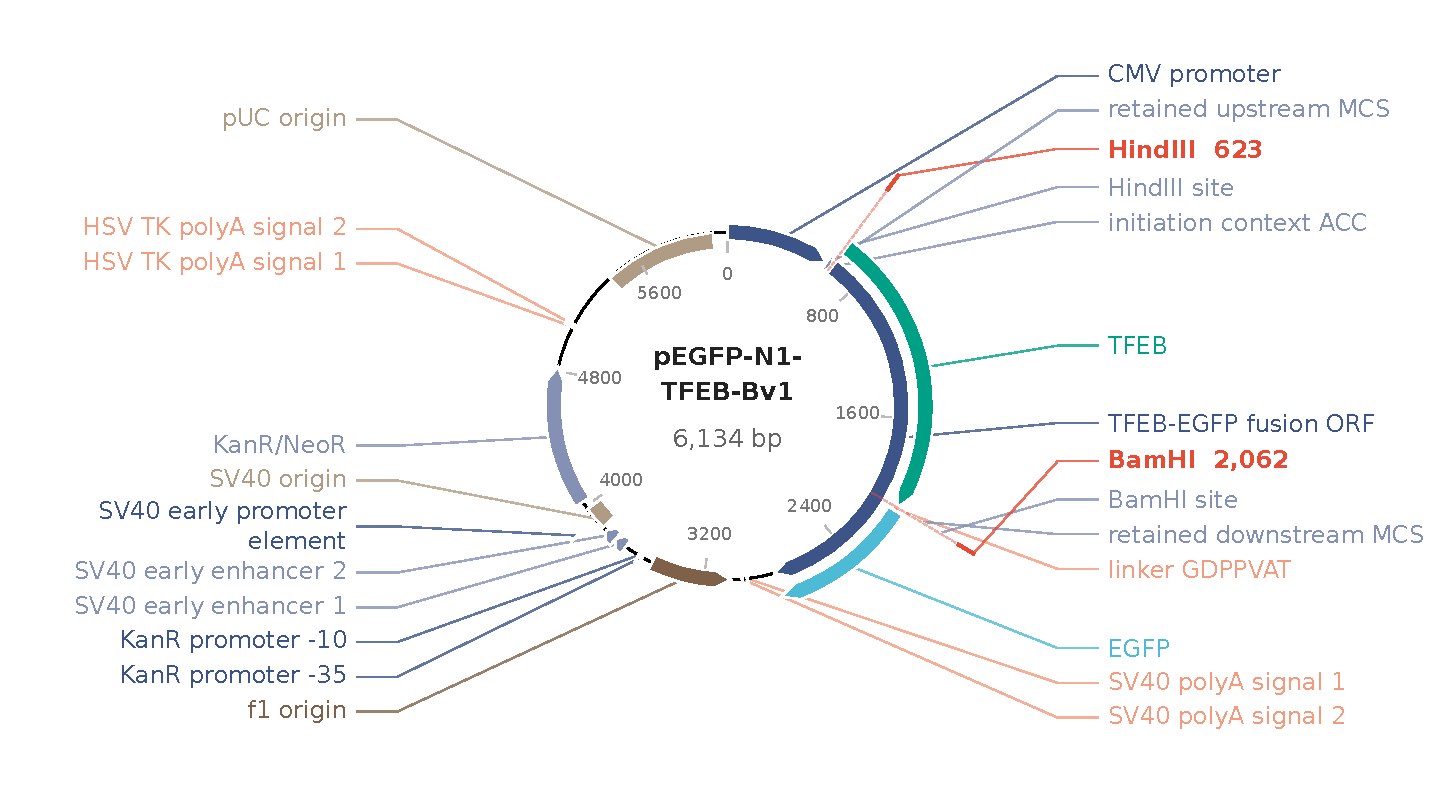
\includegraphics[width=\textwidth]{images/B/plasmid-map.pdf}
\caption{Predicted annotation map of \ConstructName{} (\ConstructBp{} bp), rendered from the accepted GenBank sequence. The complete fusion ORF overlaps its TFEB, linker and EGFP components intentionally. HindIII 623 and BamHI 2062 denote the first reference-strand nucleotide after cleavage; their recognition sequences begin at 622 and 2061, respectively. Poly(A) annotations are signal motifs, not complete processing regions. KanR applies to bacteria and Neo/G418 to mammalian selection. The pUC and SV40 origins are shown without an inferred directional arrow. No experimental observation is represented.}
\label{fig:plasmid}
\end{figure}

Cloning PCR predicts a \PCRBp{} bp product. HindIII/BamHI digestion yields a \InsertBp{} nt insert and \BackboneBp{} nt backbone by the cut-to-cut single-strand convention. Their pydna duplex spans are 1,443 and 4,699 bp, including four-base overhangs; gel sizes use the nominal single-strand lengths. Because the empty vector loses a \RemovedMCSBp{} nt MCS segment, the final length is not the intact vector length plus the undigested amplicon.

% Values transcribed from the P6-accepted expected_fragments.tsv.
Table~\ref{tab:screening} and Figure~\ref{fig:bands} summarize screening. Flanking PCR distinguishes insert-bearing candidates from empty vector. A negative orientation assay is read together with an amplification-positive control. If all orientation assays are negative in the first round, flanking-positive candidates go to sequencing. Reverse TFEB is a hypothetical challenge; incompatible-end directional ligation does not favor it.

\begin{table}[htbp]
\centering\small
\caption{Predicted screening products. All sizes are nominal bp; ``none'' means no specific product is predicted. R and S are hypothetical challenge sequences.}
\label{tab:screening}
\begin{tabularx}{\textwidth}{@{}L{3.2cm}YYY@{}}
\toprule
Sample & Flanking PCR (S-F1/S-R1) & Orientation PCR (S-F2/S-R1) & HindIII/BamHI digest \\
\midrule
Intended construct (C) & 2,605 & 2,093 & 4,695 + 1,439 \\
Empty vector (E) & 1,204 & none & 4,695 + 38 \\
Reverse TFEB (R) & 2,605 & none & 4,695 + 1,439 \\
Retained TFEB stop (S) & 2,608 & 2,096 & 4,695 + 1,442 \\
\bottomrule
\end{tabularx}
\end{table}

Flanking PCR and HindIII/BamHI digestion do not separate reversed TFEB from the intended construct, and the three-base retained-stop difference falls below gel resolution. Acceptance therefore rests on the expected digest plus actual, unambiguous, concordant bidirectional sequence across 602--2799 (2,198 nt), including both junctions, the complete fusion ORF and terminal stop. Ten primers predict usable coverage in both directions at every target base. Low-quality calls, mixed peaks, gaps and unexpected target changes are resolved under the Sanger acceptance procedure before cell assays. Figure~\ref{fig:workflow} summarizes the planned workflow and controls.


\begin{figure}[htbp]
\centering
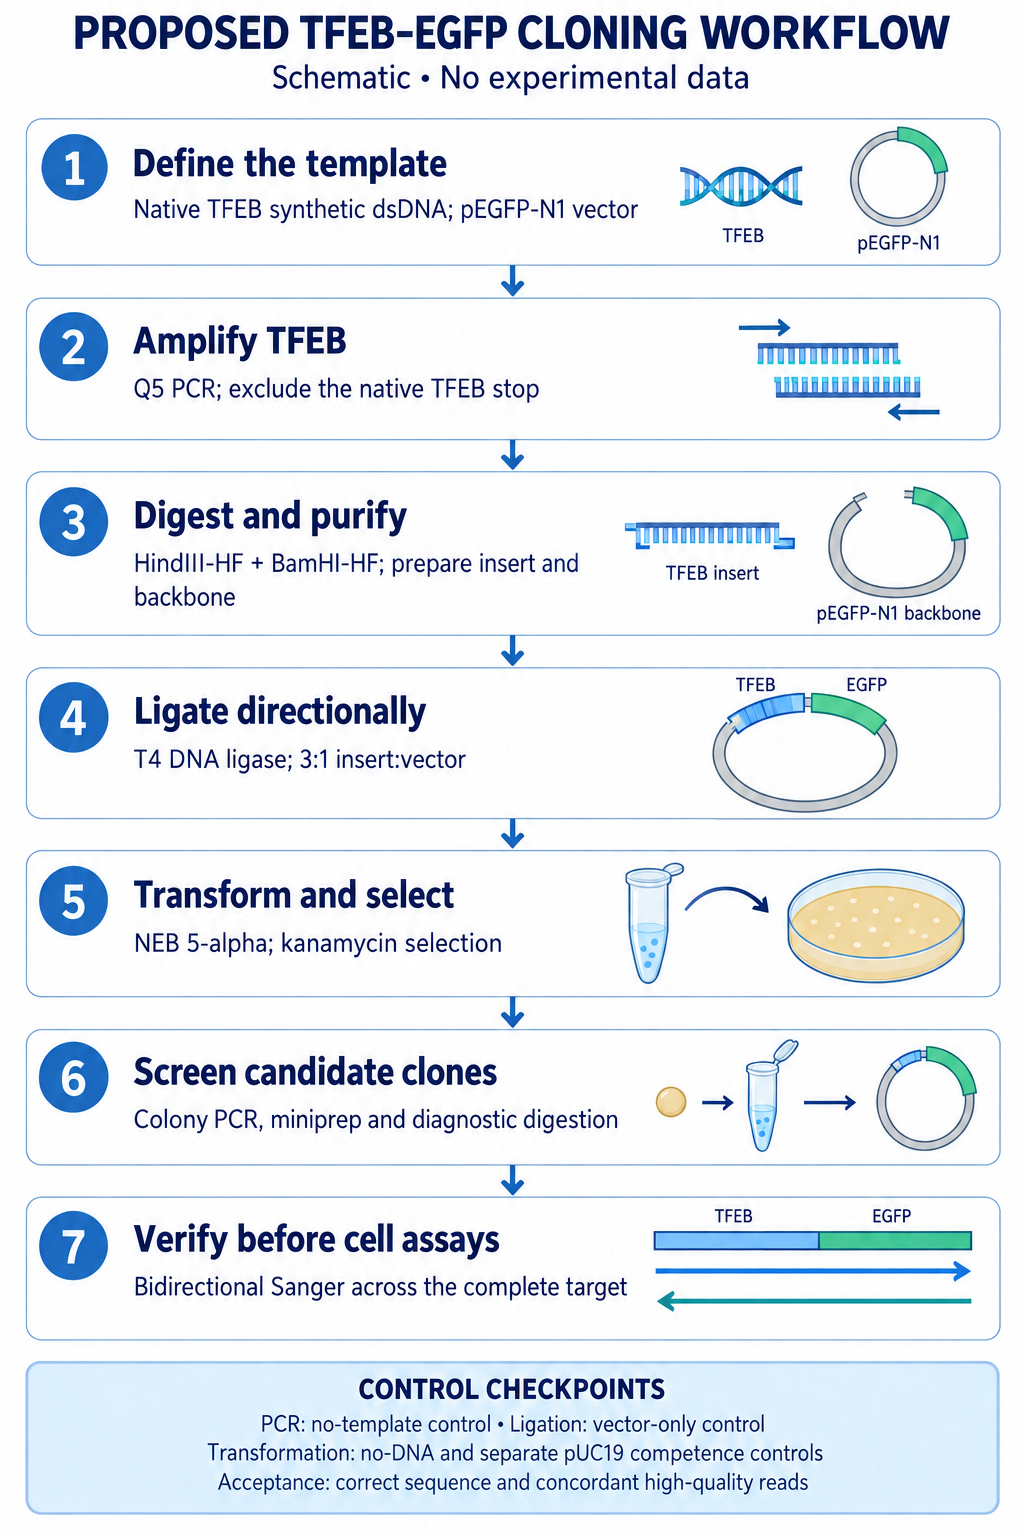
\includegraphics[width=0.92\textwidth,height=0.77\textheight,keepaspectratio]{images/B/cloning-workflow-imagegen-v2.png}
\caption{Proposed cloning workflow and control checkpoints. AI-assisted illustrations are symbolic, not exact molecular geometry, plasmid coordinates or experimental data. The full-length paired arrows summarize the intended bidirectional sequencing coverage, not observed reads. Each operation is planned; measured DNA concentrations and actual sequence quality are required before clone acceptance.}
\label{fig:workflow}
\end{figure}

\begin{figure}[htbp]
\centering
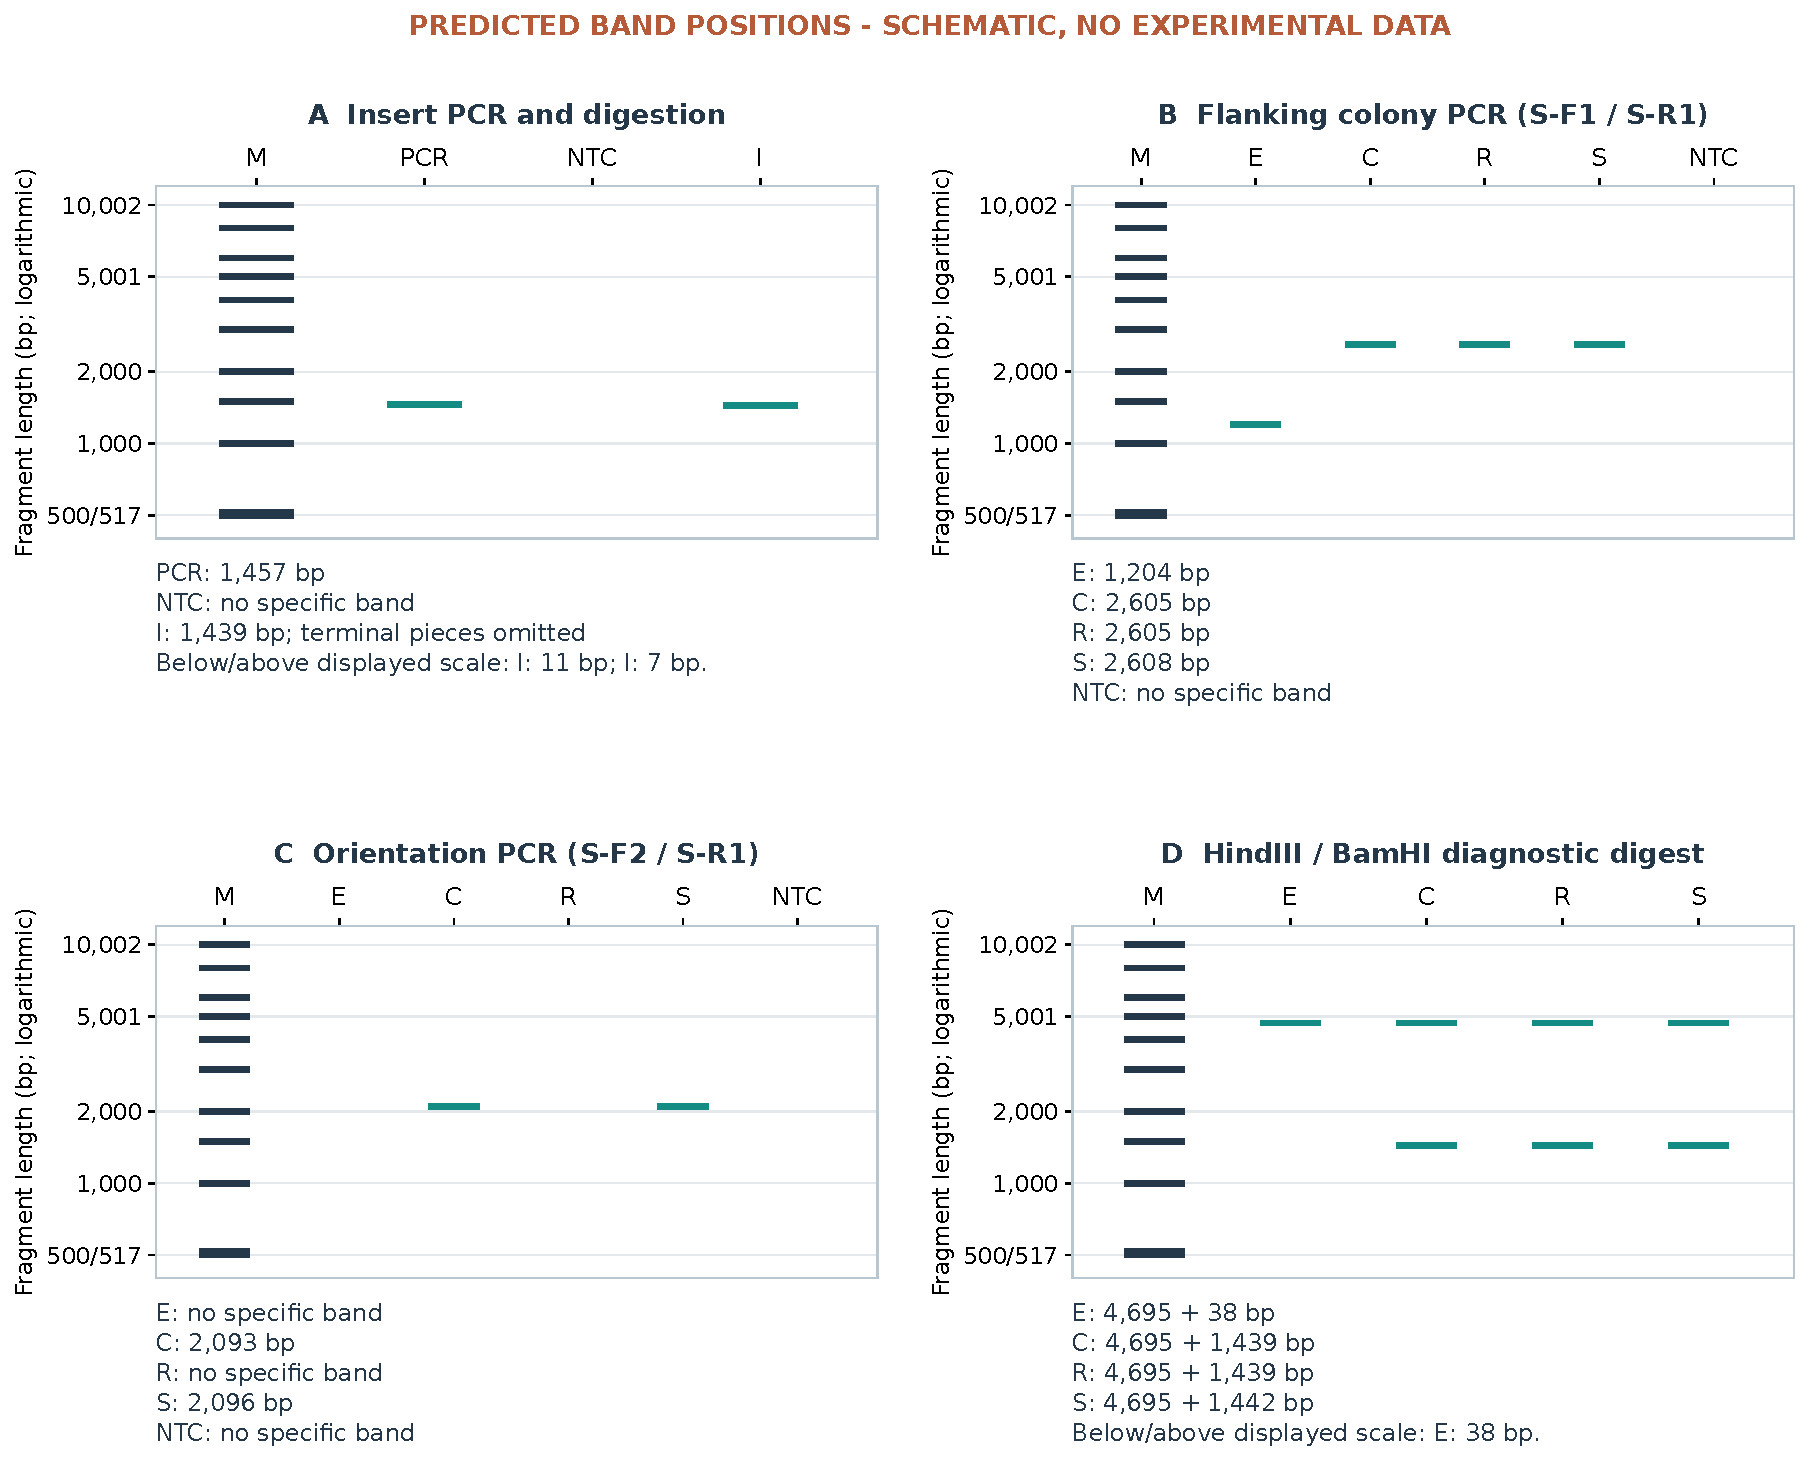
\includegraphics[width=\textwidth]{images/B/predicted-bands.pdf}
\caption{Predicted DNA-band positions, drawn as a schematic rather than an experimental gel. M: NEB N3232 ladder; PCR: tailed insert amplicon; I: digested insert; NTC: no-template control; E: empty vector; C: intended construct; R: hypothetical reverse-TFEB model; S: hypothetical retained-stop model. The 500/517 bp marker pair is not resolved~\cite{MethodM16}. The 7, 11 and 38 nt fragments fall below the displayed range. Three-base differences between C and S are not expected to resolve on the proposed 1\% gel. An empty NTC schematic means no specific product is predicted, not a guarantee of a clean experimental lane. Uncut circular DNA mobility and band intensity are not predicted.}
\label{fig:bands}
\end{figure}
\FloatBarrier

% Owner A: Ziyan Song.
\subsection{Expression and Nutrient-Dependent Localization}
The reporter is expected to show a higher nuclear-to-cytoplasmic fluorescence ratio after starvation or Torin1 treatment than in the vehicle-treated condition. An anti-GFP-reactive band consistent with the finalized fusion-protein size would support expression of the intended product.

Evidence for nutrient responsiveness will require a reproducible treatment effect across independent experiments, supported by expression and imaging controls. The magnitude and uncertainty of the localization change will be reported alongside the statistical comparison. A failure to observe redistribution would prompt checks of sequence, fusion orientation, expression level, treatment response, and imaging conditions.


\section{Discussion and Limitations}
The expanded design links construct identity, nutrient-sensitive distribution, selected regulatory sites and downstream function. Its strength comes from comparisons that separate competing explanations: matched nutrient/solvent controls, endogenous confirmation, expression titration, individual and combined site substitutions, genetic perturbation, and loss-and-rescue. A planned sequence of execution is construct acceptance, cell-assay pilot, localization/recovery confirmation, then mechanism and functional modules. Failed early quality checks are resolved before downstream interpretation.

Each control has a defined scope. EGFP-only does not prove that a TFEB fusion behaves exactly like endogenous protein. Site substitutions perturb local chemistry as well as phosphorylation potential. RPTOR/RICTOR comparisons strengthen complex attribution but require competent knockdown and may reveal indirect effects; direct phosphorylation requires a separate biochemical experiment. Recovery of N/C is net redistribution, not an independently measured export rate. TFEB knockdown and rescue can support a contribution without establishing that TFEB is the only MiT/TFE-family mediator.

Nuclear accumulation, transcription and autophagic turnover are distinct endpoints. A stress response can move TFEB into nuclei without improving degradation. Drug-induced autophagy can also involve TFEB-independent pathways. Consequently, the proposed functional conclusions require their own genetic and inhibitor controls. If those assays disagree, the conclusion is narrowed to the supported level rather than describing every endpoint as ``activation.''

The C-terminal extension adds a question beyond reproducing redistribution. Its factorial design separates tag-dependent and stimulus-dependent effects, while 3T supplies a complementary chemical perturbation. Neither alanine nor threonine substitution isolates phosphorylation from all structural consequences. Matched nuclear exposure, target engagement and phosphosite specificity are therefore necessary to interpret transcriptional differences. A null result with a wide interval remains inconclusive. The study does not claim that this exact experimental combination is unprecedented.

This remains an experimental proposal: no wet-lab clones, images, blots, qPCR measurements or flux data have been acquired. The new sequence files establish intended mutant identities, not their cellular activity. Supplier-specific reagents, siRNA targets, qPCR oligos, antibody performance and final doses/sample size require documented pilot validation. These implementation items and actual author contributions must be resolved before execution or course submission. The design can address major foreseeable objections; it cannot guarantee that every alternative mechanism has been excluded.

% Planned responsibilities supplied by the authors on October 23, 2026.
% Replace future-tense responsibilities with actual contributions at submission.
\section*{Author Contributions}
Siyuan Jiang will lead TFEB sequence retrieval, vector selection, cloning and primer design, molecular methods, plasmid and workflow diagrams, clone-verification criteria, and the related literature review. Ziyan Song will lead the abstract, biological rationale, HeLa-cell experiments, localization and expression analysis, cell-related expected results, discussion, and the related literature review. Both authors will review the construct-to-cell-assay interface and the integrated report.

\section*{AI Use Declaration}
AI assistance was used to organize the supplied outline, identify preliminary reference and construct-logic issues, and prepare the LaTeX manuscript structure. The authors will review the final scientific content, sequence design, experimental parameters, references, and contribution statement before submission.

\printbibliography[heading=bibintoc,title={References}]
\end{document}
